\documentclass[11pt,notitlepage]{article}
\usepackage{graphicx}
\usepackage[version=3]{mhchem}
\usepackage[brazilian]{babel}
\usepackage[T1]{fontenc}
\usepackage[utf8]{inputenc}
\usepackage[sfdefault]{quattrocento}
\usepackage{enumitem}
\usepackage{multicol}
\usepackage{titling}
\usepackage{titlesec}
\usepackage{lastpage}
\usepackage{indentfirst}
\usepackage{amsmath}
\usepackage{amssymb}
%\hyphenpenalty=5000
%\tolerance=5000
\setlength{\columnsep}{1cm}
\titleformat{\section}
{\normalfont\fontsize{14}{15}\bfseries}{\thesection}{1em}{}
\setlength{\columnsep}{0.5cm}
%\setlength{\columnseprule}{1pt}%
\def\columnseprulecolor{\color{black}}
\usepackage{fancyhdr}
\usepackage{parskip}
\usepackage{float}
\usepackage[left=0.25in,right=0.25in,top=0.25in,bottom=0.25in,paperwidth=7.5in,paperheight=10.62in]{geometry}
\usepackage[a4,center,noinfo]{crop}
\pagestyle{fancy}
\lhead{Caderno de questões - Parte 2}
\rhead{Prova Cognitiva Integrada 1 - M5 (2019/S2)}
%\cfoot{\thepage} Apenas o número da página no centro do rodapé
\cfoot{Página \thepage\ de \pageref{LastPage}}

% Perfeito
\titleformat{\section}
{\normalfont}
{\filright
	%\footnotesize NÃO DESCOMENTE
	\bfseries \enspace Questão \thesection\enspace}
{8pt}
{}
% fim do perfeito

% Perfeito
\titleformat{\part}[frame]
{\normalfont}
{\filright
	%\footnotesize NÃO DESCOMENTE
	\bfseries \enspace Caso Clínico \thepart\enspace}
{8pt}
{}
% fim do perfeito

\setcounter{section}{26}
\setcounter{part}{5}
\renewcommand{\headrulewidth}{0.4pt}
\renewcommand{\footrulewidth}{0.4pt} 
%\renewcommand{\thesection}{Questão \arabic{section}                                                 

\setlength{\droptitle}{-6em}     % Eliminate the default vertical space
\addtolength{\droptitle}{-6pt}   % Only a guess. Use this for adjustment

\titlespacing{\section}{0pt}{6pt}{6pt}

\title{\vspace{-5ex}}
%\title{Prova Cognitiva Integrada 1 - M6 - 2019/S1 - 05/04/2019 }
\date{\vspace{-5ex}}
\preauthor{}
\postauthor{}
\author{}

%######################
\begin{document}
%######################

\maketitle % habilita a exibição do título do documento
%\thispagestyle{empty} % Limpa definições de estilo e usa aquelas do pacote fancy

\part{José Luiz Barbosa, 37 anos, morador no bairro do Cecap, procura a UBS do seu bairro com queixa de tosse intensa e crises repetidas de falta de ar. Várias vezes procura sua Unidade Básica de saúde  referindo que gostaria apenas de fazer um aerossol, porque está com “falta de ar, tosse seca e chiado no peito” e quando coloca sua mão em seu tórax tem a sensação que esta tremendo. Ao ser acolhido pela equipe de saúde, é encaminhado para a consulta médica. Na anamnese José Luiz relata que passou a ter estes sintomas após início de trabalho numa empresa de produtos químicos. A equipe de saúde acionou o CEREST para que fizesse a inspeção da referida empresa e o estudo em conjunto da possível patologia relacionada ao trabalho. Foram solicitados exames e também fornecidos medicamentos para melhora dos sintomas, sendo estes medicamentos previstos na REMUME.}
\vspace{0.5cm}

\section{O ato de ouvir o paciente está relacionado a qual instrumento utilizado pela Política de Humanização?}
\noindent\makebox[\linewidth]{\rule{\textwidth}{0.5pt}}
\noindent\makebox[\linewidth]{\rule{\textwidth}{0.5pt}}
\vspace{0.5cm}

\section{Os fatores de risco para a saúde e segurança do trabalhador podem ser classificados em cinco grandes grupos, qual deles está relacionado a patologia desenvolvida pela José Luiz?}
\noindent\makebox[\linewidth]{\rule{\textwidth}{0.5pt}}
\noindent\makebox[\linewidth]{\rule{\textwidth}{0.5pt}}
\vspace{0.5cm}

\section{Quais os blocos que compõem a assistência farmacêutica no SUS?}
\noindent\makebox[\linewidth]{\rule{\textwidth}{0.5pt}}
\noindent\makebox[\linewidth]{\rule{\textwidth}{0.5pt}}
\noindent\makebox[\linewidth]{\rule{\textwidth}{0.5pt}}
\vspace{0.5cm}

\section{O paciente, ao final da consulta, solicita o atestado médico para ser apresentado na empresa onde trabalha para justificar sua ausência neste dia devido a seu estado de saúde. O médico elabora o atestado, mas coloca, por engano, a data do dia anterior. Ao deixar a unidade, o Sr José Luiz se atenta deste fato e, na recepção, solicita à enfermeira para que seja feita a correção pelo médico que o atendeu. Este médico se recusa a elaborar outro atestado e rasura a data do atestado anteriormente elaborado, corrigindo para a data correta. Sobre os documentos médicos, assinale a alternativa correta:   }
\begin{multicols}{2}
	\setlength{\columnseprule}{0pt}
	\begin{enumerate}[label=(\alph*)]
		\item neste caso, em que é somente uma rasura sem importância, ou seja, a data correta, o médico agiu corretamente e isso não é passível de futuras consequências.
		\item O atestado médico, por ser um documento legal, não pode ser rasurado, ainda que seja em coisa mínima, já que, segundo a ética médica, só deve ser emitido documento médico quando efetivamente se pratica o ato profissional que o justifique e que corresponda exatamente à verdade. 
		\item Segundo o código de ética em vigor atualmente, durante a internação o prontuário médico deve ser legível e, no momento da alta do paciente, não há necessidade de elaboração, pelo médico assistente, do sumário de alta a ser entregue ao paciente, mas se o fizer, cabe algumas rasuras devido a erros comuns.
		\item O médico que atendeu este paciente pode deixar de dar o atestado a este paciente, já que ele está na unidade de saúde pública e, por ser órgão público, não é obrigado a emitir atestados quando o paciente assim o solicita em consulta médica.
	\end{enumerate}
\end{multicols}
%\vspace{0.5cm}

\part{Paciente Maria Oliveira, 78 anos de idade, chega para ser atendida na Unidade de Saúde, queixa-se de fraqueza, dor nas costas e no abdome e dois dias apresenta diarreia e vômito. Como antecedente relata hipertensão arterial e diabetes mellitus. Apresenta frequência respiratória de 32 mpm, FC = 110 bpm, P= 108 bpm, aferido na artéria radial e PA= 90x50 mmHg, temperatura axilar de 38,5º C. A paciente tem história de infarto do miocárdio de parede lateral do ventrículo esquerdo há 3 meses, confirmado por eletrocatrodiogramas.}
\vspace{0.5cm}

\section{Baseado na localização anatômica da lesão miocárdica e seu suprimento sanguíneo, qual artéria coronária sofreu a obstrução súbita? }
\begin{multicols}{2}
	\setlength{\columnseprule}{0pt}
	\begin{enumerate}[label=(\alph*)]
		\item artéria coronária descendente anterior esquerda
		\item artéria coronária direita
		\item artéria coronária circunflexa esquerda
	\end{enumerate}
\end{multicols}
\vspace{0.5cm}

\section{A distribuição da lesão isquêmica do miocárdio descrita anteriormente pode ser classificada como:}
\begin{multicols}{2}
	\setlength{\columnseprule}{0pt}
	\begin{enumerate}[label=(\alph*)]
		\item transmural
		\item subendocárdica
		\item global
		\item parcial
		\item temporária
	\end{enumerate}
\end{multicols}
\vspace{0.5cm}

\part{Homem de 47 anos, caminhoneiro e prestador de serviço em uma usina de açúcar e álcool da região, é levado à UPA – Araraquara, após acidente com seu caminhão. No estabelecimento foi constatada a existência de uma fratura óssea na perna direita, sendo necessária a cirurgia corretiva e, também, foi constatado sangramento moderado, causando ligeira queda nos níveis pressóricos arteriais. Foi admitido na unidade de clinica cirúrgica após procedimento cirúrgico no braço esquerdo fraturado e na perna esquerda, apresenta uma laceração em sua testa. Está com infusão intravenosa (RS-500 ml) com cateter periférico flexível n.20 na veia mediana do cotovelo na fossa antecubital direita e foi colocada uma meia de compressão pneumática na perna direita inferior. Recebe oxigênio através de máscara facial simples. Após avaliação dos exames de controle foi indicada reposição sanguínea com concentrado de hemácias, devido ao quadro de anemia aguda, mas o paciente se recusa a aceitar o procedimento, afirmando ser adepto da corrente religiosa “Testemunha de Jeová”.}
\vspace{0.5cm}

\section{O Paciente pode recusar receber o tratamento:}
\begin{multicols}{2}
	\setlength{\columnseprule}{0pt}
	\begin{enumerate}[label=(\alph*)]
		\item se estiver em risco de morte;
		\item se estiver consciente e orientado e em risco de morte;
		\item em qualquer circunstância, independe do quadro clínico, diagnóstico e prognóstico;
		\item apenas se for plenamente capaz e não houver risco de morte;
		\item alegando o princípio da beneficência e sua condição religiosa, mesmo estando em risco de morte iminente.
	\end{enumerate}
\end{multicols}
\vspace{0.5cm}

\section{Quais são os dois princípios bioéticos, segundo o principialismo, evolvidos no caso acima?}
\noindent\makebox[\linewidth]{\rule{\textwidth}{0.5pt}}
\noindent\makebox[\linewidth]{\rule{\textwidth}{0.5pt}}
\vspace{0.5cm}

\part{Afonso, 47 anos, casado, bancário, mora com a esposa e 1 filha, hipertenso há 15 anos (pressão arterial de repouso: 160x110 mm de Hg) e portador de litíase renal Refere ser tabagista há 23 anos. Também comentou que teve diagnóstico de miocardite linfocítica aos 23 anos de idade. Antecedentes familiares: A mãe de falecida de infarto agudo do miocárdio e pai aos 80 anos de morte por câncer. Atualmente encontra-se internado na Santa Casa de Araraquara por angina típica. \textbf{Dados antropométricos} Circunferência da cintura: 120 cm; P= 78 Kg;   A=1,62m. \textbf{Dados dietéticos}: Consumo familiar mensal: sal – 2 pacotes; óleo: 6 latas; açúcar: 3 Kg. Temperos: utiliza os do tipo concentrados (caldo Knnor®, Sazon®). Modo de preparo dos alimentos: geralmente fritos (empanados) ou refogados. Pele do frango e gordura visível da carne: nunca retirados antes das preparações. Consumo De carne vermelha diariamente (2 x /dia); Consumo de água: 2 copos/dia (requeijão). Consumo de refrigerantes: diariamente – coca zero. Uso de produtos industrializados (embutidos e enlatados). Nega intolerâncias alimentares.}
\vspace{0.5cm}

\section{Qual dos seguintes agentes infecciosos tem sido associado mais frequentemente ao desenvolvimento da patologia referida aos 23 anos de idade? }
\begin{multicols}{2}
	\setlength{\columnseprule}{0pt}
	\begin{enumerate}[label=(\alph*)]
		\item Coxsackie vírus
		\item ECHO
		\item Influenza
		\item Citomegalovírus
		\item Todas as alternativas estão corretas
	\end{enumerate}
\end{multicols}
\vspace{0.5cm}

\section{Em função do quadro do paciente, quais alimentos e/ou componentes alimentares apresentados nos dados dietéticos estão relacionados ao quadro de urolitiase?  }
\noindent\makebox[\linewidth]{\rule{\textwidth}{0.5pt}}
\noindent\makebox[\linewidth]{\rule{\textwidth}{0.5pt}}
\noindent\makebox[\linewidth]{\rule{\textwidth}{0.5pt}}
\vspace{0.5cm}

Ao atender o Sr Afonso, você fez 4 orientações dietéticas a ele:\\
\noindent\makebox[\linewidth]{\rule{\textwidth}{0.5pt}}
\noindent\makebox[\linewidth]{\rule{\textwidth}{0.5pt}}
\noindent\makebox[\linewidth]{\rule{\textwidth}{0.5pt}}
\noindent\makebox[\linewidth]{\rule{\textwidth}{0.5pt}}
\vspace{0.5cm}

O Sr Afonso é hipertenso, em sua consulta, você orientou o consumo de sódio de \underline{\hspace{2cm}} mg que equivale a \underline{\hspace{2cm}} g de sal de cozinha. O máximo de sódio que os indivíduos adultos devem consumir é de \underline{\hspace{2cm}} mg.
\vspace{0.5cm}

\part{Eurípedes, 52 anos, comerciante, casado, diagnostico de Insuficiência Renal Crônica, taxa de filtração glomerular > 60, PA de 15X12 mmHg. Seus exames bioquímicos revelam hipertrigliceridemia, discreta hipercreatinemia, sem presença de diabetes. Refere que seu peso habitual era de 60 Kg antes da descoberta da IRC e sente-se inapetente. \textbf{Dados antropométricos}: A = 1,65m; P= 54 Kg. \textbf{Dados dietéticos}: Faz 3 refeições ao dia: desjejum, almoço e jantar. Desjejum = 1 copo de leite integral com achocolatado. Almoço = consumo eventual de verduras folhosas, 2 colheres de arroz, 1 file grande de carne, 1 doce, especialmente chocolates. No jantar geralmente faz uso de pão com frios e refrigerantes ou sopas prontas em pó. Tem preferência por massas. Não tem hábito de consumir frutas, a não ser a carambola antes da descoberta da IRC. Uso do saleiro à mesa.}
\vspace{0.5cm}

\section{Proponha uma terapia combinada para o tratamento de Eurípides. Justifique farmacologicamente sua resposta. }
\noindent\makebox[\linewidth]{\rule{\textwidth}{0.5pt}}
\noindent\makebox[\linewidth]{\rule{\textwidth}{0.5pt}}
\noindent\makebox[\linewidth]{\rule{\textwidth}{0.5pt}}
\noindent\makebox[\linewidth]{\rule{\textwidth}{0.5pt}}
\noindent\makebox[\linewidth]{\rule{\textwidth}{0.5pt}}
\noindent\makebox[\linewidth]{\rule{\textwidth}{0.5pt}}
\noindent\makebox[\linewidth]{\rule{\textwidth}{0.5pt}}
\noindent\makebox[\linewidth]{\rule{\textwidth}{0.5pt}}
\noindent\makebox[\linewidth]{\rule{\textwidth}{0.5pt}}
\noindent\makebox[\linewidth]{\rule{\textwidth}{0.5pt}}
\noindent\makebox[\linewidth]{\rule{\textwidth}{0.5pt}}
\noindent\makebox[\linewidth]{\rule{\textwidth}{0.5pt}}
\noindent\makebox[\linewidth]{\rule{\textwidth}{0.5pt}}
\vspace{0.5cm}

\section{Quais efeitos podem ser esperados da interação dos fármacos associados na terapia proposta na questão anterior? Identifique os fármacos e as interações.}
\noindent\makebox[\linewidth]{\rule{\textwidth}{0.5pt}}
\noindent\makebox[\linewidth]{\rule{\textwidth}{0.5pt}}
\noindent\makebox[\linewidth]{\rule{\textwidth}{0.5pt}}
\noindent\makebox[\linewidth]{\rule{\textwidth}{0.5pt}}
\noindent\makebox[\linewidth]{\rule{\textwidth}{0.5pt}}
\noindent\makebox[\linewidth]{\rule{\textwidth}{0.5pt}}
\noindent\makebox[\linewidth]{\rule{\textwidth}{0.5pt}}
\noindent\makebox[\linewidth]{\rule{\textwidth}{0.5pt}}
\noindent\makebox[\linewidth]{\rule{\textwidth}{0.5pt}}
\noindent\makebox[\linewidth]{\rule{\textwidth}{0.5pt}}
\noindent\makebox[\linewidth]{\rule{\textwidth}{0.5pt}}
\noindent\makebox[\linewidth]{\rule{\textwidth}{0.5pt}}
\noindent\makebox[\linewidth]{\rule{\textwidth}{0.5pt}}
\vspace{0.5cm}

\section{Qual a provável explicação para o resultado do exame bioquímico de creatinina de Eurípedes?}
\begin{multicols}{2}
	\setlength{\columnseprule}{0pt}
	\begin{enumerate}[label=(\alph*)]
		\item os níveis séricos de creatinina não são marcadores sensíveis da função renal em doença renal crônica, principalmente no início da perda de função dos rins ou fase de insuficiência renal funcional ou leve.
		\item a ureia é o primeiro marcador a aumentar, a creatinina demora um pouco mais.
		\item possivelmente a dosagem de creatinina sofreu alguma interferência in vitro com cefalosporinas ou N-acetilcisteína, dipirona, corpos cetônicos, proteínas plasmáticas ou bilirrubinas. 
		\item possivelmente o paciente não realizou um preparo adequado para a obtenção da amostra.
		\item a realização intensa de exercícios e refeições com elevado conteúdo de carne podem ter sido a causa de interferência nesse exame.
	\end{enumerate}
\end{multicols}
\vspace{0.5cm}

\section{Baseado na descrição acima, ofereça ao Sr. Euripedes 4 orientações dietéticas que ele deverá seguir para conseguir um bom controle pressórico. Não serão aceitas orientações quanto a exercício físico, tabagismo ou consumo de bebidas alcoólicas. O tratamento dietético é essencial na prevenção das complicações decorrentes da insuficiência renal crônica. Acerca da relação entre dieta e progressão da doença renal crônica, avalie as asserções a seguir.:
	I.A restrição proteica é uma intervenção dietética indicada para pacientes com insuficiência renal crônica\\
	II. A restrição proteica promove a redução de produtos nitrogenados tóxicos, retardando o ritmo de progressão da doença\\
	III. Na dieta hipoproteica convencional oferece-se cerca de 0,6 g/kg/dia de proteina para manter o balanço hidrogenado, sendo que 80\% dessa proteína é de origem vegetal\\
	IV. Na dieta muito hiperproteica oferece-se proteína de origem vegetal (15 a 20\% do VCT) suplementada com aminoácidos essenciais para corrigir sintomas urêmicos}
\begin{multicols}{2}
	\setlength{\columnseprule}{0pt}
	\begin{enumerate}[label=(\alph*)]
		\item I, II corretas
		\item II, III corretas
		\item I, III corretas
		\item III, IV corretas
		\item I, IV corretas
	\end{enumerate}
\end{multicols}
\vspace{0.5cm}

\section{A Insuficiência Renal Crônica (IRC) é clinicamente caracterizada pela perda progressiva das funções renais que se traduzem pela presença de sinais como hiperpotassemia entre outros. Para esta situação recomenda-se diminuir a quantidade de potássio dos alimentos. Oriente o Sr Eurípedes sobre alimentos fonte de potássio }
\noindent\makebox[\linewidth]{\rule{\textwidth}{0.5pt}}
\noindent\makebox[\linewidth]{\rule{\textwidth}{0.5pt}}
\noindent\makebox[\linewidth]{\rule{\textwidth}{0.5pt}}
\noindent\makebox[\linewidth]{\rule{\textwidth}{0.5pt}}
\vspace{0.5cm}

\part{C.A.S., sexo feminino, casada, doméstica, obesa e residente na cidade de Araraquara, em 2009, aos 55 anos de idade, durante exame médico de rotina apresentou valores de pressão arterial de 150/96 mmHg e os resultados laboratoriais abaixo:\\ 
	Exames laboratoriais em 2009: Glicemia de jejum = 255 mg/dL; Colesterol total = 220 mg/dL; HDL-colesterol = 28 mg/dL; Triglicérides = 375 mg/dL; Creatinina sérica = 0,7 mg/dL e Ureia = 20 mg/dL. Tais exames foram repetidos e confirmaram-se valores de glicemia e triglicérides anormais.\\
	Em 2017, a paciente foi encaminhada ao oftalmologista, que diagnosticou microaneurisma em vãos de retina, sugestivo de retinopatia, tendo sido realizada laserterapia. Recentemente, em 2019, após 10 anos, aos 65 anos de idade, ao exame físico realizado por seu endocrinologista, apresentou um peso de 106 kg, pressão arterial de 170/112 mmHg, com frequência cardíaca de 72 batimentos por minuto, e os seguintes exames laboratoriais:\\
	Exames laboratoriais em 2019: Glicemia de jejum = 150 mg/dL; HbA1c = 6,5\%; Colesterol total = 184 mg/dL; HDL-colesterol = 30 mg/dL; Triglicérides = 450 mg/dL; Creatinina sérica = 1,8 mg/dL; Ureia = 66 mg/dL.\\
	Para realizar os exames laboratoriais solicitados pelo clínico em sua última consulta, C.A.S. acordou bem cedo e dirigiu-se ao laboratório no centro da cidade, realizando uma caminhada de 20 minutos. No laboratório, após ter apresentado seus documentos pessoais e a solicitação de exame, recebeu da atendente um protocolo com numeração. Durante a coleta da amostra de sangue precisou apresentar novamente os seus documentos pessoais e não recebeu nenhum questionamento quanto ao seu preparo para a realização dos exames. As amostras de sangue foram obtidas por punção venosa e acondicionadas em estante, ficando expostas à luz e temperatura ambiente por um período de 4 horas até serem processadas e armazenadas.\\
	(Valores de referência: Colesterol total: desejável < 190 mg/dL, HDL-colesterol: desejável > 40mg/dL; Triglicérides: desejável < 150 mg/dL; LDL-colesterol: desejável ou baixo < 130 mg/dL; Creatinina sérica: mulheres = 0,53 a 0,99 mg/dL e homens = 0,70 a 1,2mg/dL; Ureia = 15 a 40 mg/dL). }
\vspace{0.5cm}

\section{A partir dos resultados dos exames de C.A.S. (2019), quais alimentos e/ou preparações você orientaria a eliminar da dieta, relacionando com o perfil lipídico e suas frações? }
\noindent\makebox[\linewidth]{\rule{\textwidth}{0.5pt}}
\noindent\makebox[\linewidth]{\rule{\textwidth}{0.5pt}}
\noindent\makebox[\linewidth]{\rule{\textwidth}{0.5pt}}
\noindent\makebox[\linewidth]{\rule{\textwidth}{0.5pt}}
\vspace{0.5cm}

\section{Aos 55 anos de idade, C.A.S. foi diagnosticada diabética, dislipêmica e hipertensa. Qual foi o critério utilizado pelo clínico para diagnosticar e confirmar diabetes? }
\begin{multicols}{2}
	\setlength{\columnseprule}{0pt}
	\begin{enumerate}[label=(\alph*)]
		\item duas glicemias de jejum $\geqslant$ 126 mg/dL
		\item duas glicemias de jejum $\geqslant$ 200 mg/dL
		\item glicemia de 2 h $\geqslant$ 140 mg/dL no TOTG
		\item glicemia de 2 h $\geqslant$ 200 mg/dL no TOTG
		\item glicemia de 2 h entre 140 a 199 mg/dL no TOTG
	\end{enumerate}
\end{multicols}
\vspace{0.5cm}

\section{Além da retinopatia diabética, atualmente o paciente apresenta outra complicação crônica decorrente do diabetes. Essa complicação crônica poderia ter sido identificada no início para o estabelecimento de terapia que impedisse a sua progressão. Nesse caso, o teste laboratorial utilizado para identificá-la seria:}
\begin{multicols}{2}
	\setlength{\columnseprule}{0pt}
	\begin{enumerate}[label=(\alph*)]
		\item Hemoglobina glicada
		\item Frutosamina
		\item Microalbuminúria
		\item Peptídeo C
		\item Pesquisa de corpos cetônicos
	\end{enumerate}
\end{multicols}
\vspace{0.5cm}

\section{O teste laboratorial de Hemoglobina glicada A1c (HbA1c), utilizado no controle de tratamento do paciente diabético, nos últimos anos, passou a ser utilizado como prova diagnóstica. Quanto à sua utilização como prova diagnóstica é correto afirmar: }
\begin{multicols}{2}
	\setlength{\columnseprule}{0pt}
	\begin{enumerate}[label=(\alph*)]
		\item pode ser substituída pelos testes laboratoriais de Hemoglobina glicada total ou Hemoglobina glicada A1
		\item está condicionada ao uso da metodologia analítica de cromatografia líquida de alta performance (HPLC) ou outro método certificado pelo National Glycohemoglobin Standardization Program (NGSP)
		\item está condicionada apenas ao uso da metodologia analítica de cromatografia líquida de alta performance (HPLC)
		\item pode ser substituída em alguns casos pelo teste laboratorial de Frutosamina
		\item pode ser realizada através de qualquer metodologia analítica confiável e previamente testada
	\end{enumerate}
\end{multicols}
\vspace{0.5cm}

\section{Quais as frações de colesterol obtida em 2019 segundo Martin et al.?}
%### Descri��o breve ###
\begin{figure}[H]
	\centering
	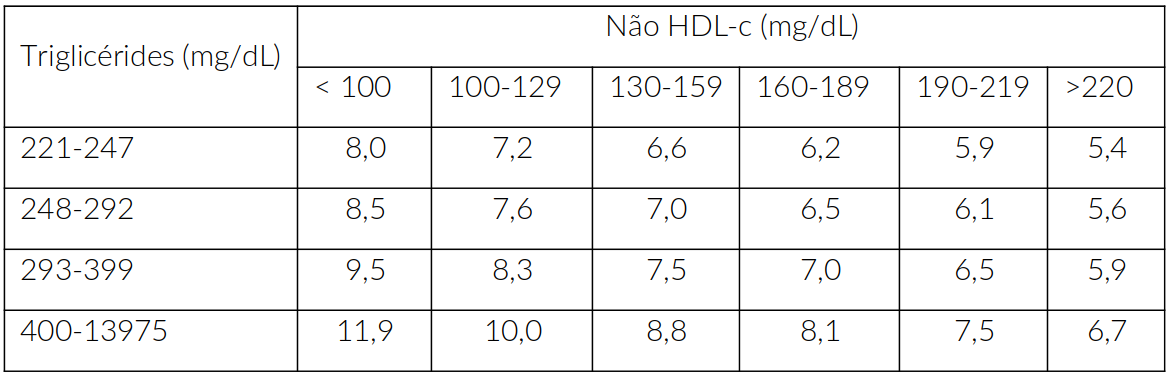
\includegraphics[scale=0.32]{q46.png}
	\caption{Valores utilizados para determinação do Col VLDL segundo Martin et al. }
	\label{fig:link de chamada}
\end{figure}
%###########
\begin{multicols}{2}
	\setlength{\columnseprule}{0pt}
	\begin{enumerate}[label=(\alph*)]
		\item Col HDL = 30 mg/dL; \\Col VLDL = 55,6; \\Col LDL = 133,4 mg/dL
		\item Col HDL = 30 mg/dL; \\Col VLDL = 51,1; \\Col LDL = 138,9 mg/dL
		\item Col HDL = 30 mg/dL; \\Col VLDL = 37,8; \\Col LDL = 152,2 mg/dL
		\item Col HDL = 30 mg/dL; \\Col VLDL = 60; \\Col LDL = 130 mg/dL
		\item Col HDL = 30 mg/dL; \\Col VLDL = 45; \\Col LDL = 145 mg/dL
	\end{enumerate}
\end{multicols}
\vspace{0.5cm}

\section{A realização de atividade física produziu alteração principalmente na dosagem de:}
\begin{multicols}{2}
	\setlength{\columnseprule}{0pt}
	\begin{enumerate}[label=(\alph*)]
		\item proteínas totais
		\item colesterol total
		\item bilirrubinas
		\item glicemia
		\item triglicerídeos
	\end{enumerate}
\end{multicols}
\vspace{0.5cm}

\section{A solicitação de documentos pessoais e a entrega de protocolo foram medidas realizadas pelo laboratório para evitar, respectivamente, os seguintes erros laboratoriais:}
\begin{multicols}{2}
	\setlength{\columnseprule}{0pt}
	\begin{enumerate}[label=(\alph*)]
		\item de identificação como outra pessoa e de coleta de materiais
		\item de identificação como outra pessoa e de entrega de resultados
		\item de identificação como outra pessoa e de troca voluntária de amostras
		\item de coleta de materiais e de homônimos
		\item de homônimos e de entrega de resultados
	\end{enumerate}
\end{multicols}
\vspace{0.5cm}

\section{O acondicionamento dado à amostra de sangue de C.A.S. até o processamento e armazenamento, possivelmente:}
\begin{multicols}{2}
	\setlength{\columnseprule}{0pt}
	\begin{enumerate}[label=(\alph*)]
		\item não produziu nenhuma alteração nos analitos
		\item desnaturou os anticorpos presentes e reduziu a atividade enzimática
		\item produziu hemólise e trombólise
		\item alterou a taxa sérica de eletrólitos
		\item degradou bilirrubinas
	\end{enumerate}
\end{multicols}
\vspace{0.5cm}

\section{Falecimento de uma mulher com traumatismo cranioencefálico como consequência de disparo intencional de arma de fogo.  É internada na unidade de terapia intensiva, apresentou parada cardiorrespiratória e teve o óbito verificado pelo médico plantonista, após o insucesso das manobras de reanimação. Como classificaria esse óbito? }
\begin{multicols}{2}
	\setlength{\columnseprule}{0pt}
	\begin{enumerate}[label=(\alph*)]
		\item causa natural
		\item causa externa
		\item hospitalar
		\item sem assistência médica
		\item desconhecido
	\end{enumerate}
\end{multicols}
\vspace{0.5cm}

\section{Em ferimentos incisos, a cauda de saída é, geralmente:}
\begin{multicols}{2}
	\setlength{\columnseprule}{0pt}
	\begin{enumerate}[label=(\alph*)]
		\item mais alongada e superficial
		\item mais curta e profunda
		\item mais alongada e profunda
		\item mais curta e superficial
		\item mais profunda e aberta
	\end{enumerate}
\end{multicols}
\vspace{0.5cm}

\section{O médico legista realiza pericias:}
\begin{multicols}{2}
	\setlength{\columnseprule}{0pt}
	\begin{enumerate}[label=(\alph*)]
		\item a pedido das partes
		\item mediante solicitação através de advogados diretamente ao mesmo
		\item por requisição da autoridade policial ou ministério público
		\item a pedido dos familiares da vitima
		\item quando requisitadas por autoridade policial ou judiciária
	\end{enumerate}
\end{multicols}
\vspace{0.5cm}

%###############################################################################
% Final do documento
\end{document}
%####################